\documentclass[main.tex]{subfiles}
\graphicspath{{image/}}

\begin{document}

\chapter{チャプター}\label{chapter}

本稿では、沼津高専\footnote{独立行政法人\;国立高等専門学校機構\;沼津工業高等専門学校}にて全学生に配布されている学生証についてできるだけ開設する。
また、学生証を用いたシステム開発の手助け等を目的として執筆している。%

\section{セクション}

本物は見せられないので忠実に再現した画像を用いる.\par

\begin{figure}[H]
    \centering
    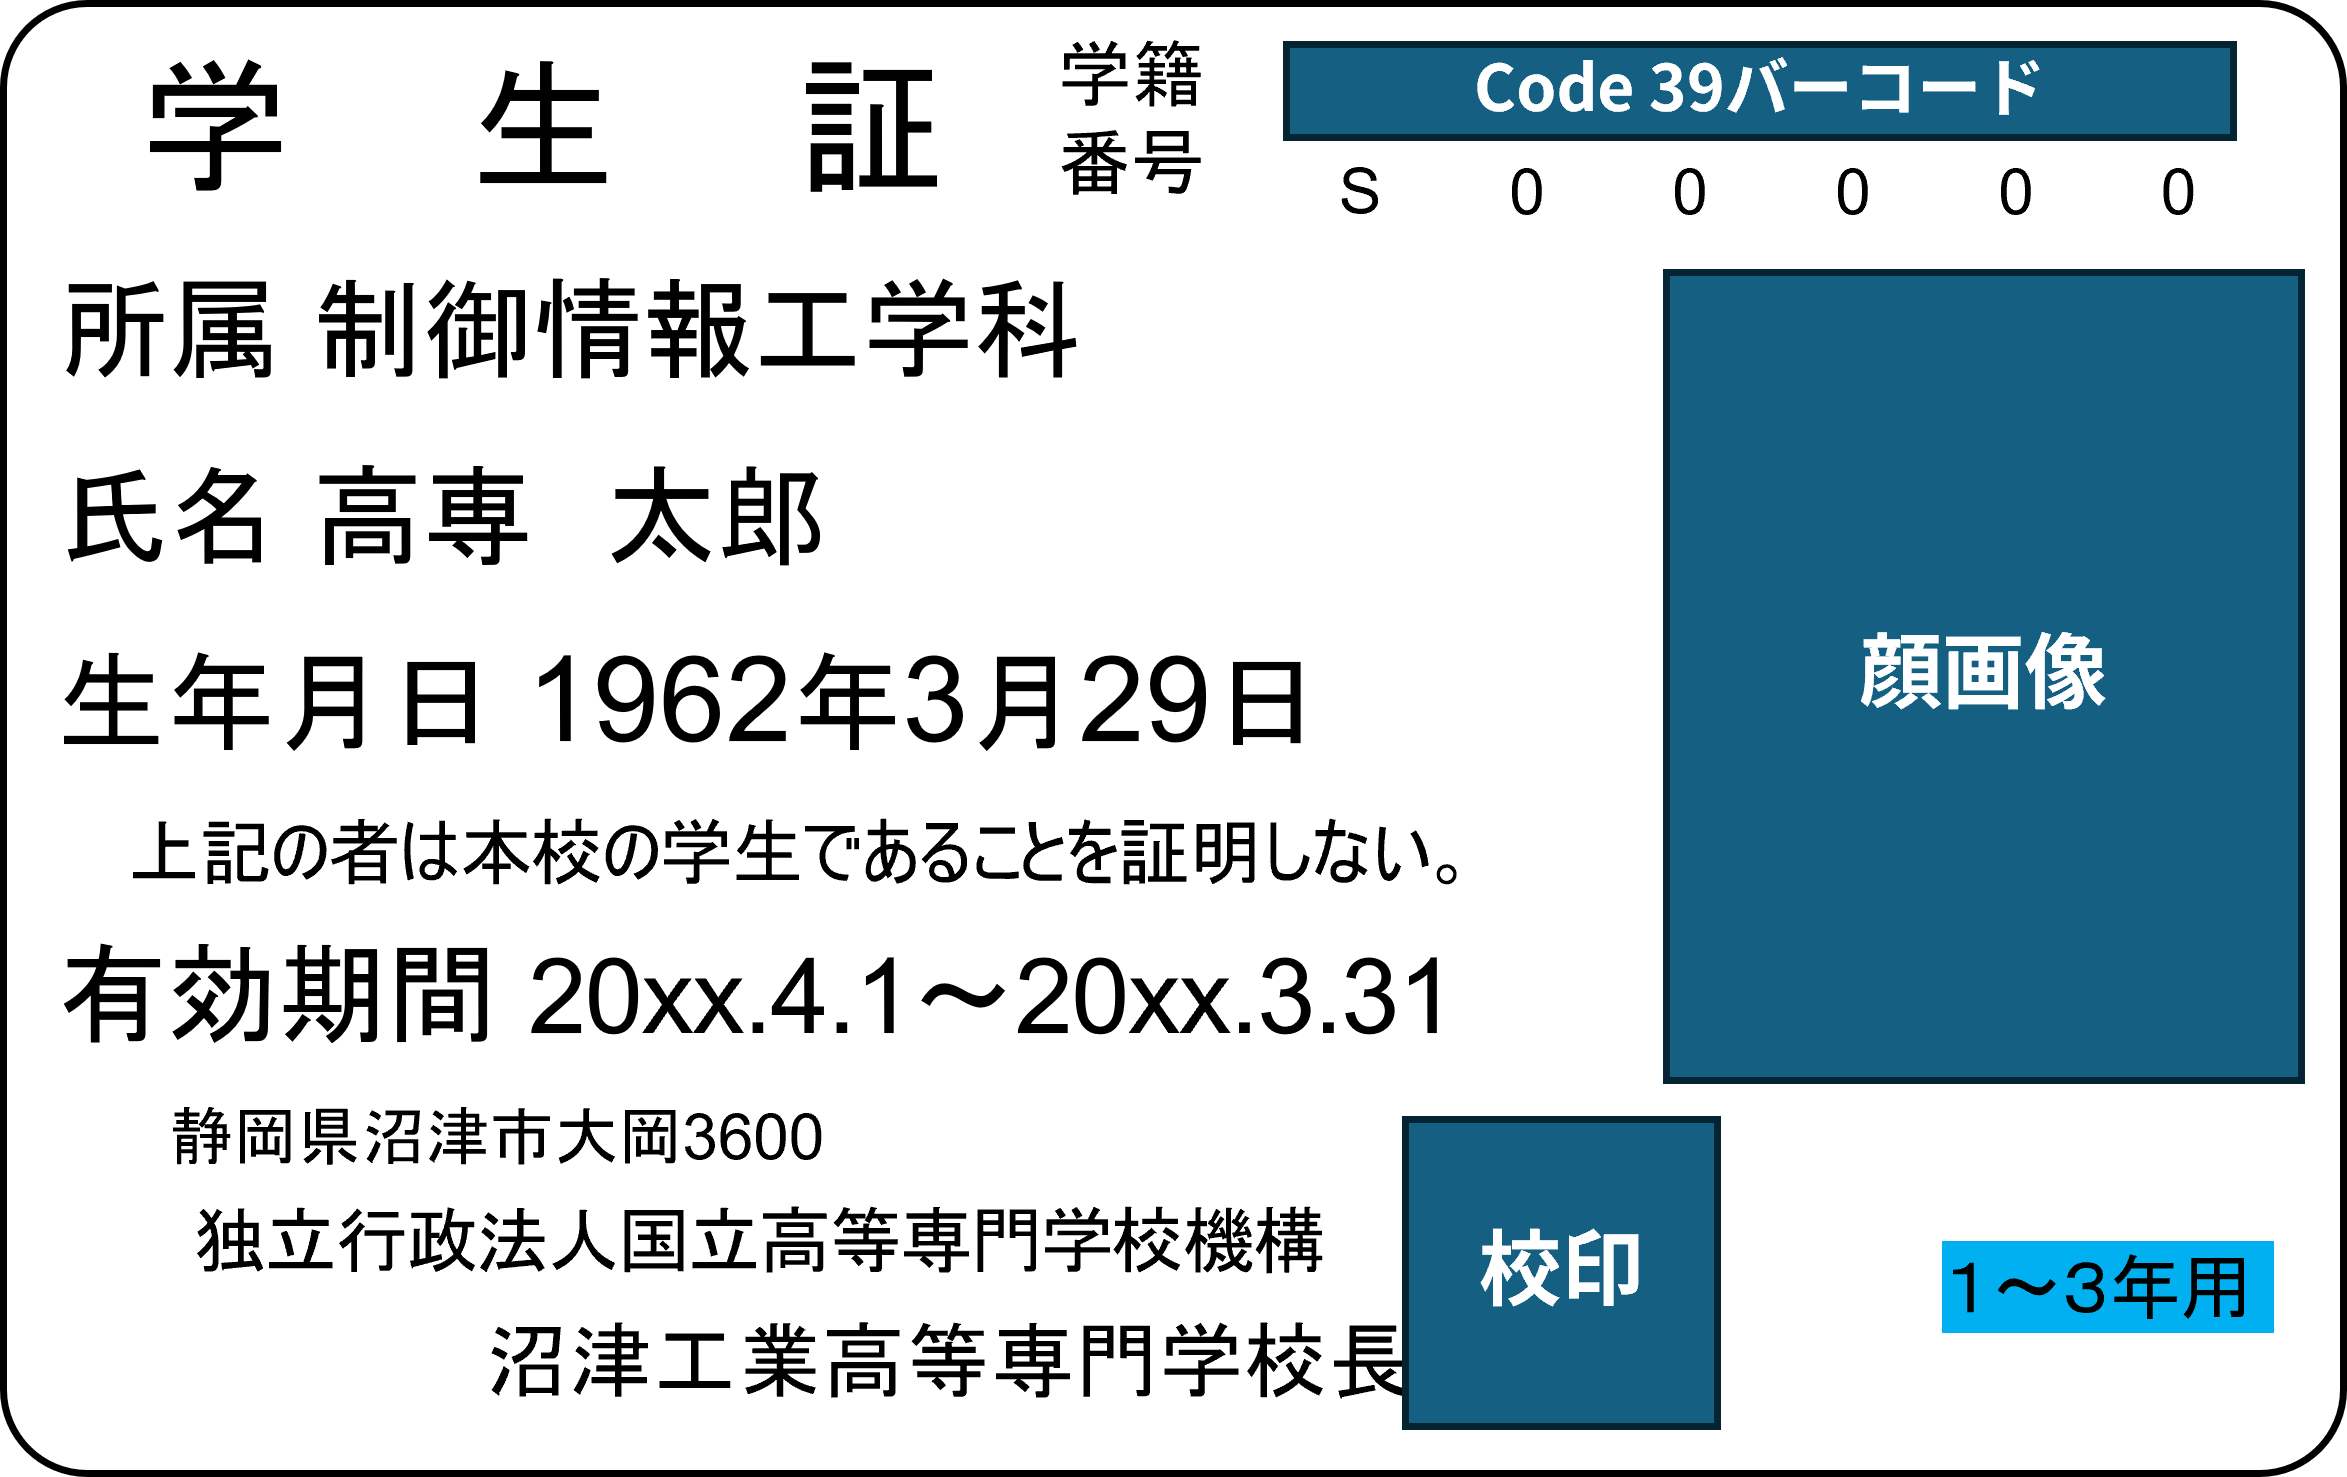
\includegraphics[width=85.60truemm]{image/front.png}
    \caption{画像サンプル}
    \label{fig:gakusei_front}
\end{figure}

フォントは数字部分はArial, 日本語部分はMS UI Gothicが使われていると思われる.

サイズはクレジットカードなどと同じ53.98x85.60mmとなっている.
\LaTeX が仕事をしていれば実寸大になっているはず.

pagerefは、\mypageref{chapter}、refは\myref{章}{chapter}のように表す

\begin{itemize}
    \item 機械工学科
          \begin{itemize}
              \item 電気電子工学科
                    \begin{itemize}
                        \item 電子制御工学科
                              \begin{itemize}
                                  \item 制御情報工学科
                                  \item 物質工学科
                              \end{itemize}
                    \end{itemize}
          \end{itemize}
\end{itemize}

\begin{description}
    \item[これがdescriptionのタイトル]
    これが内容
    \item[\ttfamily I: 全割り込み許可]\mbox{}\\
    改行する時はこんな感じ
\end{description}

\clearpage

定積分の定義は以下のようになります多分。

\begin{equation*}
    \int_a^b f(x) \,dx = \lim_{n \to \infty} \sum_{i=1}^{n} f(x_i^*) \Delta x_i
\end{equation*}

\subsection{サブセクション}

\subsubsection{サブサブセクション}

ここに \texttt{inline code} が入ります。

以下がソースコードです。

\begin{sourcecode}
int main(void)
{
    // 日本語だよ
    // This is comment!
    printf("Hello world!");
}
\end{sourcecode}

以下のように書くとファイルからソースコードを表示できます。

\begin{codebox}
    \lstinputlisting[]{sourcecode/test.cpp}
\end{codebox}

\clearpage

これがコールアウトです。
\begin{note}
    \texttt{\$ npm run dev}を実行しないと、処理が開始されません。必ず実行するようにしてください。
\end{note}

\begin{warn}
    \texttt{\$ npm run dev}を実行しないと、処理が開始されません。必ず実行するようにしてください。
\end{warn}

\begin{caution}
    \texttt{\$ npm run dev}を実行しないと、処理が開始されません。必ず実行するようにしてください。
\end{caution}

\texttt{simplebox}環境は以下のように使います

\begin{simplebox}
\textbf{関数 \texttt{llvm::IRBuilderBase::CreateRet}}
\tcblower
\begin{verbatim}
ReturnInst *CreateRet(Value *V)
\end{verbatim}
\end{simplebox}

\appendix

\chapter{彼女作るンゴ}

\section{結論}

無理。

\newpage

\end{document}
